\section{Evaluation} \label{sec:eval}

We have evaluated our system on a 64-bit Dell server running Ubuntu
server 8.04 with kernel version 3.2.9. We used one Flash based SSD and
one SATA HDD. The SSD is an Intel SSDSA2CW300G3 2.5-inch with 300G
capacity. The SATA disk is a Maxtor 7L250S0 3.5-inch SATA HDD. Its
capacity is 250GB and its rotational speed is 7200 rpm. The code and
benchmark results are publicly available at
https://github.com/brianchenming/mris.

\subsection{Measure drives}

Firstly, we measured the two storage devices used in our benchmarks.
The results we got support our argument that Flash is good in random
I/O while HDD is not bad in sequential I/Os. We formated both devices
using Ext4. We remount devices before each benchmark to make sure that
all disk caches are dropped. The devices were measured using
Filebench~\cite{filebench-web}. Random read and write were measured
using Filebench built-in workloads \texttt{randomread} and
\texttt{randomwrite}; Sequential read and write were measured using
Filebench built-in workloads \texttt{singalstreamread} and
\texttt{singalstreamwrite}.

\begin{figure}[t]
\begin{centering}
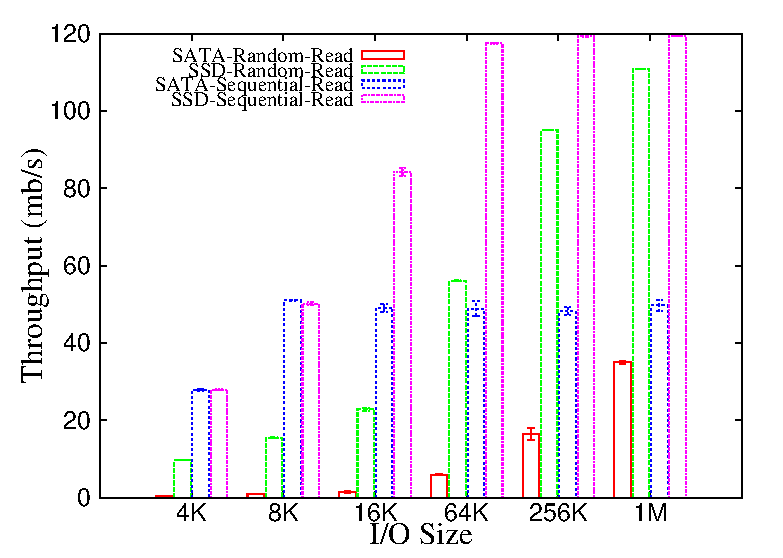
\epsfig{file=figures/ssd_vs_sata_read.eps,width=1.00\linewidth}
\caption{Read performance of SSD and HDD}
\label{fig:driveread}
\end{centering}
\end{figure}

The performance of read operations are presented in
Figure~\ref{fig:driveread}. All benchmarks are performed for 3 times,
and the standard deviation of the 3 runs are shown as error bar in
figures. The results are stable and most error bars are imperceptible
or negligible. As we can see in Figure~\ref{fig:driveread}, SSD is
much better than that of HDD for random read for small I/O sizes. SSD
is 23.1$\times$ faster than HDD when I/O size is 4K, and 18.4$\times$
faster when I/O size is 8K. However, the speed advantage drops to
8.4$times$ and 4.8$times$ when the I/O size grows to 64K and 256K.
This is because disk head seek happens less frequently as I/O size
increases. Specifically, the HDD read throughput is 0.4mb/s with an
I/O size of 4K. This agrees with the 9ms average read time shown in
the HDD's specification.  

For sequential read, the most interesting observation is that HDD
provided the same throughput as SSD when I/O size is 4K and 8K. HDD
throughput stop grow after 8K, whereas SSD throughput grows until
256K. 8K and 256K are the points when HDD and SSD achieve their
respective maximum bandwidth.

\begin{figure}[t]
\begin{centering}
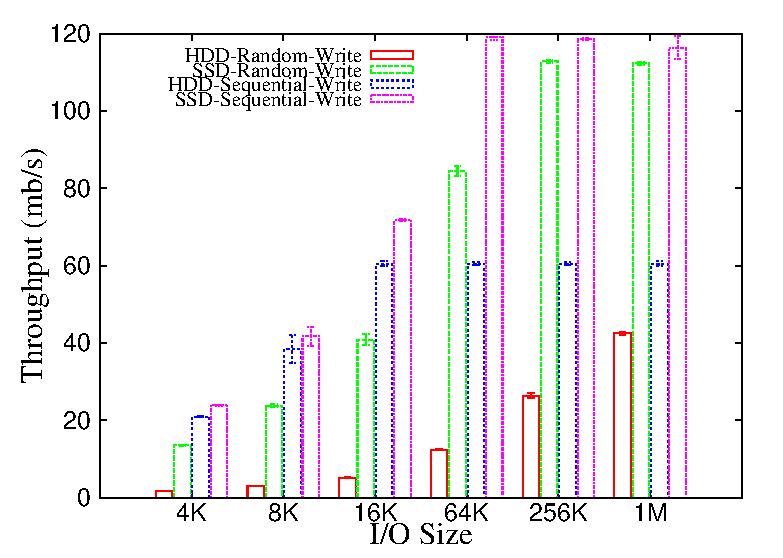
\epsfig{file=figures/ssd_vs_sata_write.eps,width=1.00\linewidth}
\caption{Write performance of SSD and HDD}
\label{fig:drivewrite}
\end{centering}
\end{figure}

The performances of write operations are presented in
Figure~\ref{fig:drivewrite}. They present similar trend as of read.
When I/O size is small (i.e. 4K, 8k, or 16k), SSD performs much better
than HDD for random write, but their performance have no significant
difference for sequential write. When I/O size becomes large,
throughput of both drives are capped by their maximum bandwidth.
However, we noticed that HDD performs better for write than for read.
This is because the HDD has a 16MB internal cache, which is more
helpful for write than for read.

Above-mentioned results will serve as baselines of throughput for our
further benchmarking. They also validate our design premise that SSD
performs much better than HDD for random I/Os and HDD performs well
for sequential I/Os.

\subsection{Wikipedia Image Workload}

\begin{figure}[t]
\begin{centering}
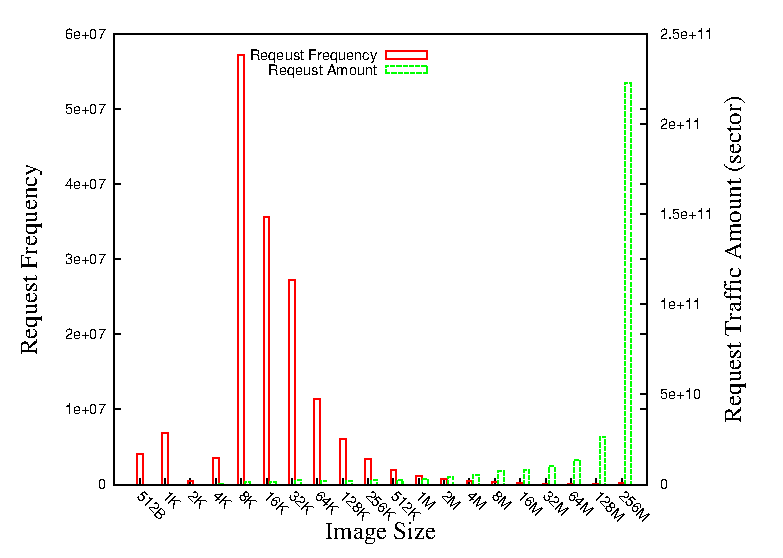
\epsfig{file=figures/wiki-image.eps,width=1.00\linewidth}
\caption{Image Requests to Wikipedia of January 2012}
\label{fig:wikiimage}
\end{centering}
\end{figure}

To study the size-tiered property in workloads, we analyzed the
requests of images made to Wikipedia site.  Wikipedia is the #5
website in the world~\cite{wikipedia-web}, serving 492 million people
every month~\cite{wikipedia-foundation}. It can reflect workloads of
many large websites.

Figure~\ref{fig:wikiimage} presents the requests of images made in
January 2012. They are extraced from request log files, which are
available at
http://dumps.wikimedia.org/other/pagecounts-raw/2012/2012-01/. We
extract requests of objects with a suffix of jpg, png, or gif, then
round up their sizes into power of 2. The frequency of images of
different sizes is counted and plotted in Figure~\ref{fig:wikiimage}.
All images larger than 256M is counted in the 256M bin. The first
observation from Figure~\ref{fig:wikiimage} is that the request image
of different sizes vary widely.  Particularly, images of sizes between
$(4, 64]$ KB are most popular. They sum to 81.58\% of the total number
of image requests. Moreover, 94.57\% of the requests are for images
smaller than or equal to 128KB. Despite the fact that small images
(<=128KB) are the absolute majority in term of request numbers, the
traffic (size$\times$frequency) introduced by them is just 2.96\% of
the total. Although not all the requests make their way to the storage
layer because of memory cache (such as Memcached~\cite{memcached}).
This salient size-tiered property of requests still makes size-tiered
storage a close match for multi-resolution image workloads.

\subsection{Micro Benchmarks}

We first show micro benchmark results on simple workloads of
sequential and random read and write of MRIS. To demonstrate the
benefits of multi-tier system, we experimented every workload on three
different setups. 

\subsection{Facebook Workloads}

1. 17 of Ran R on three setups

2. RR workload of different ratios on hybrid.

To evaluate the green target, we created virtual devices using our
target, performed I/Os on the devices using \texttt{dd}, and compared
them with devices created by the linear target.  Both types of virtual
devices have the same configuration. They are 1G large, with the first
256M comes from the SSD and the rest comes from the SATA. The extent
size of the green device is 4K by default. The mapping table of the
linear and green virtual devices are presented in Figure
\ref{fig:dmtable} (a) and (b), wherein \texttt{/dev/sdd} is the SSD
and \texttt{/dev/sdc} is the SATA disk. 

To start with, we considered the best scenario first. It happens when
linear devices are accessing the SATA disk whereas green devices map
all I/Os onto the SSD.  In this experiment, we still measured the time
elapsed to read/write 1G of data from the green and linear device
using the Linux \texttt{dd} command.  We also confined the address
space covered by the I/Os to be within 256M so that the green disk can
map all of them on the SSD without migration.  We also make sure
offsets of all the I/Os are larger than 256M so that all I/Os are
served by the SATA for the linear device. However, in the case of the
green device, all I/Os are served by SSD thanks to the flexible
mapping mechanism.  

\subsection{Wikipedia Workloads}

We present the results in Figure \ref{fig:best}.  For read, the green
device is more than 3 times faster for all 7 different I/O sizes.
Particularly, when the I/O size is 64K and 256K, the speedup is more
than 7 and 5 times respectively. This suggests the green device can be
a good fit for workloads containing most I/Os of these sizes. However,
for write, the green device does not exhibit any advantage over the
linear device. This is the same as the comparison between writes of
the SSD and SATA disk. In fact, the whole Figure \ref{fig:best} and
Figure \ref{fig:ssd_vs_sata} are very close to each other. This is
exactly what we are expecting because, in the best scenario, the
linear device works using only the SATA disk, whereas the green device
works using only the SSD.


%%%%%%%%%%%%%%%%%%%%%%%%%%%%%%%%%%%%%%%%%%%%%%%%%%%%%%%%%%%%%%%%%%%%%%%%%%%%%%
%% For Emacs:
% Local variables:
% fill-column: 70
% End:
%%%%%%%%%%%%%%%%%%%%%%%%%%%%%%%%%%%%%%%%%%%%%%%%%%%%%%%%%%%%%%%%%%%%%%%%%%%%%%
%% For Vim:
% vim:textwidth=70 noai nocin nosi
%%%%%%%%%%%%%%%%%%%%%%%%%%%%%%%%%%%%%%%%%%%%%%%%%%%%%%%%%%%%%%%%%%%%%%%%%%%%%%
% LocalWords:  
